% =============================================================================
% cs-logic-circuit.tex — Combinational logic circuit (half adder)
%
% Shows: a half adder — S = A XOR B, C = A AND B — with labelled inputs,
% gates, and outputs. The canonical first circuit in any digital-logic or
% computer-organization course.
% Compiles standalone via: xelatex cs-logic-circuit.tex
%
% Use for: digital logic, computer organization (adders/ALU), Boolean algebra.
% Extend to a full adder by adding a second XOR/AND pair and an OR gate.
% =============================================================================

\documentclass[border=4pt]{standalone}
\usepackage{tikz}
\usetikzlibrary{arrows.meta, positioning, circuits.logic.US, calc}

\definecolor{wire}{HTML}{1A1A1A}
\definecolor{gate-border}{HTML}{012169}
\definecolor{label-gold}{HTML}{B9975B}

\tikzset{
  circuit logic US,
  every circuit symbol/.style={draw=gate-border, thick, fill=white},
  wire/.style={draw=wire, thick},
  pin-label/.style={font=\small},
  % Junction dot for a fan-out point
  junction/.style={circle, fill=wire, minimum size=3.4pt, inner sep=0pt}
}

% -----------------------------------------------------------------------------
% Diagram: Half adder. A and B fan out to an XOR gate (sum) and an AND gate
% (carry).
% Coordinates: (x, y)
%   Input A rail at y = 1.4 ; input B rail at y = 0.6
%   XOR gate centred at (4.0, 1.6)  -> output S at (5.6, 1.6)
%   AND gate centred at (4.0, -0.2) -> output C at (5.6, -0.2)
%   Fan-out junctions at x = 1.2 (A) and x = 1.8 (B)
% Vertical drop lines run at x = 1.2 / 1.8 down to the AND-gate input rails at
% y = 0.1 / -0.5, which are BELOW every gate body — no wire crosses a gate
% (P7a). Input/output labels sit left/right of their wire ends, never on them
% (P7b).
% -----------------------------------------------------------------------------

\begin{document}
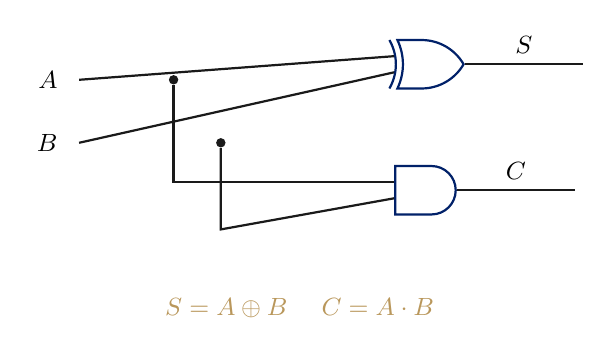
\begin{tikzpicture}

  % ---- Input labels -------------------------------------------------------
  \node[pin-label, left] at (-0.15, 1.4) {$A$};
  \node[pin-label, left] at (-0.15, 0.6) {$B$};

  % ---- Gates --------------------------------------------------------------
  \node[xor gate, inputs={nn}, anchor=input 1] (XOR) at (4.0, 1.7) {};
  \node[and gate, inputs={nn}, anchor=input 1] (AND) at (4.0, 0.1) {};

  % ---- Input rails into the XOR gate --------------------------------------
  \draw[wire] (0, 1.4) -- (XOR.input 1);
  \draw[wire] (0, 0.6) -- (XOR.input 2);

  % ---- Fan-out junctions ---------------------------------------------------
  \node[junction] (Ajoin) at (1.2, 1.4) {};
  \node[junction] (Bjoin) at (1.8, 0.6) {};

  % ---- Drop lines down to the AND gate ------------------------------------
  \draw[wire] (Ajoin) -- (1.2, 0.1)  -- (AND.input 1);
  \draw[wire] (Bjoin) -- (1.8, -0.5) -- (AND.input 2);

  % ---- Outputs -------------------------------------------------------------
  \draw[wire] (XOR.output) -- node[above, pin-label] {$S$} ++(1.5, 0);
  \draw[wire] (AND.output) -- node[above, pin-label] {$C$} ++(1.5, 0);

  % ---- Equations (placed clear of all wires, below the circuit) -----------
  \node[pin-label, align=left, text=label-gold] at (2.8, -1.5)
        {$S = A \oplus B$ \quad $C = A \cdot B$};

\end{tikzpicture}
\end{document}
